
%%This is a very basic article template.

%%There is just one section and two subsections.

\documentclass[12pt]{article}

\usepackage[slovak]{babel}
\usepackage[utf8]{inputenc}
\usepackage{amsmath}
%%\usepackage[dvipdfm]{graphicx}
\usepackage{graphicx}
\usepackage{bmpsize}
\usepackage{pdfpages}
\usepackage{wrapfig}
\usepackage{setspace}
\usepackage[top=2.54cm, bottom=2.54cm, left=3.5cm, right=2.0cm]{geometry}

\setstretch{1.5}

\begin{document}

\title{Rozpoznávanie dobravných značiek}

\author{Mário Kapusta}
%% titulka s informaciami
\maketitle
\thispagestyle{empty}
\clearpage

%% astrakt
\begin{abstract}
V praci sme sa zaoberali
\end{abstract}
\clearpage

%% zaciatok prace
\section{Počítačové videnie}
Nejaký obkec o počítačovom videní
\subsection{História počítačového videnia}
Niečo krátke o histórii počítačového videnia
\subsection{Hlavné témy počítačového videnia}
Obkec o rozdelení počítačového videnia a rôznych odvetviach venovania
\subsubsection{Transformácia}
Niečo o trnaformácii.
\subsubsection{Filtrovanie a kompresia}
Niečo o kompresii.
\subsubsection{Vylepšovanie obrazu}
Niečo o vylepšovaní obrazu.
\subsubsection{Rozpoznávanie objektov}
Niečo o rozpoznávaní objektov
\subsubsection{Pozíciovanie}
Niečo o rozpoznávaní poziciovani
\subsection{Technológie}
Niečo o o technológiách rozpoznávania vo všeobecnosti
\subsubsection{OpenCV}
Niečo o opencv - textik k tomu:
http://simplecv.tumblr.com/post/19307835766/opencv-vs-matlab-vs-simplecv
\subsubsection{Matlab}
Niečo o matlabe
\subsubsection{SimpleCV}
Niečo o simplecv

\section{Rozpoznávanie ojektov}

\section{OpenCV, Android a Java}
Cieľom je vypracovať komplexný návrh riešenia pre vyhľadávanie a rozpoznávanie dopravného značenia a taktiež vytvoriť funkčnú aplikáciu, ktorá
bude schopná rozpoznať zvislé dopravné značenia.
\subsection{Funkcionalita OpenCV}
budem opisovat najpouzivanejsie funkcie, co robia a ake algoritmy sa v nich pouzivaju
\subsubsection{cvtColor}
\subsubsection{Canny}
\subsubsection{HoughLinesP}
opisat nieco o houghovej transformacii
\subsubsection{GaussianBlur}
\subsubsection{inRange}
\subsubsection{threshold}
\subsubsection{bitmapToMat}
\subsubsection{findContours}
\subsubsection{boundingRect}
\subsubsection{drawContours}
\subsubsection{contourArea}
\subsubsection{fitEllipse}

\section{Návrh riešenia}
Po dôkladnom naštudovaní literatúry a potrebných algoritmov je našim cieľom vyhotoviť riešenie, ktoré by dokázalo detekovať zvislé dopravné značenia.
Návrh bude pozostávať z návrhu algoritmov, návrhu objektov a návrhu užívateľského prostredia.
\subsection{Návrh algoritmov}
Ako metódu rozpoznávania som si zvolil detekciu dopravného značenia podľa tvaru a farby. 
Algoritmy ktoré som navrhol, sú postavené na princípe rozpoznania farebného rozhrania hľadaného objektu a následné detekovanie potrebného tvaru.
Pri opise som sa zameral na detekciu značiek, ktoré sú na cestách najviac početné.
Na cestách prevládajú dopravné značenia, ktoré sú červenej a modrej farby. Z tvarov prevládajú kruhy a trojuholníky.
Samotné rozpoznanie bolo uskutočnené pomocou neurónových sietí. Táto metóda je najlepšia na počítačové učenie objektov.
Na rozdiel od detekcie dopravného značenia, pre riešenie neurónových sietí použijeme už existujúcu knižnicu.
\subsubsection{Návrh algoritmu pre detekciu farby}
%%TODO Spravenie vyvojoveho/stavoveho diagramu
Ako prvý algoritmus som si vybral detekciu červenej farby. Pre detekciu farieb sa v literatúre odporúča najprv previesť vstup na farebný model HSV. 
Vstup prichádza vo farebnom formáte RGB. Farebný model HSV je jeden z dvoch najpoužívanejších valcovo súradnicových reprezentácii bodov pre RGB model.
\cite{hsl_hsv_wiki_en}
\linebreak
\linebreak
- Na začiatok by sa mal vstup(bitmapa) konvertovať na binárnu maticu.
\linebreak
\linebreak
- Najväčšia výhoda dopravného značenia je, že je silne kontrastné od ostatného prostredia.
Túto vlastnosť môžeme perfektne využiť v náš prospech a pomocou pomocou rozmazania obrazu, môžeme dosieliť to,
že sa zbavíme slabších kontú hneď na začiatku. V OpenCV je pre rozmazávanie obrazu na výber viacero metód,
no my použijeme matódu \emph{GaussianBlur}, ktorá už názvom prezrádza použitie známeho filtra \emph{Gaussian blur}
\linebreak
\linebreak
- Keďže sa snažíme dostať náš vstupný obraz do formátu HSV, o ktorú sa stará funkcionalita \emph{cvtColor} 
potrebujeme mu nastaviť vstup tak, aby obraz vedel bez problémov spracovať. 
Keďže na väčšine mobilných zariadení prichádza do zariadenia obraz vo formáte RGBA, ďalší krok bude nepríklad konvertovanie formátu RGBA na formát RGB.
\linebreak
\linebreak
- Ďalej bude nasledovať samotná konverzia obrazu do HSV pomocou už spomínanej metódy \emph{cvtColor}.
\linebreak
\linebreak
- Ďalší krok bude spracovať každý kanál farebného modelu HSV samostatne. Ako prvý spracujeme \emph{Hue} kanál, ktorý sa stará o farebný odtien každého pixelu.
\emph{Hue} Farba sa v tomto kanáli určuje podľa stupňov. 
Primárne sa začína na stupni 0$^\circ$, čo predstavuje zelenú farbu, postupne prechádza do modrej,
ktorá sa nachádza na 120$^\circ$ stupňoch z kade prechádza cez červenú na 240$^\circ$ a keďže je to model kruhový, vracia sa do zelenej na 360$^\circ$.
Pomocou funkcie \emph{inRange} by nemal byť problém určiť rozhranie stupňov, ktoré sme schopný akceptovať ako hľadanú farbu pre hľadané naše dopravné značenia.
Ďalší kanál je \emph{Saturation}, ktorý predstavuje sýtosť farby. Táto sýtosť sa vyjadruje v percentách, kde 0\% predstavuje šedú a 100\% je plne sýta farba.\cite{hsv_wiki_cz} 
V našom prípade je postacuje metóda \emph{threshold}. Posledný kanál \emph{Value} vyjadruje hodnotu jasu.
Keďže v praxi znamená znižovanie jasu pridávanie čiernej do základnej farby,
pre hľadanie červenej farby na dopravnom značení nie je potrebné s týmto kanálom pracovať, lebo červená farba použitá na dopravných značeniach je pomerne svetlá.
Pri hľadaní modrej je túto farbu potrebné trochu stmaviť a tak použijeme opäť funkciu \emph{threshold}.
\linebreak
\linebreak
- Na koniec potrebujeme dostať len kontúry hľadanej farby. 
Najpr si budeme musieť spojiť jednotlivé kanály späť do jednej binárnej matice použitím metódy \emph{Canny}. 
Po tomto kroku by nám mali ostať len čierny obraz a biele škvrny predstavujúce červenú farbu v požadovanom rozsahu.
Z týchto bielych objektov, budeme potrebovať len okraje a tak použijeme metódu \emph{findContours}, ktorá sa postará o to, že dostaneme pole kontúr z celého obrazu.
S týmito kontúrami potom ďalej pracujeme a rozoznávame z nich hľadané útvary.
\subsubsection{Návrh algoritmu pre detekciu kruhov}
- Pri detekcii dopravného značenia v tvare kruhu, je dôležité počítať s tým, že nehľadáme úplný kruh. Kruhové dopravné značenia sú vyrábané ako dokonalý kruh,
no pri ich rozpoznávaní si je potrené uvedomiť, že na objekt sa pozeráme z rôznych uhlov. Táto skutočnosť nám prináša do prolematiky dôležitý fakt,
že v skutočnosti to nie sú kruhy čo hľadáme, ale sú to elipsy. Celý algoritmus je možné vidieť na orázku č. \ref{hladanie_kruhov}
\linebreak
\linebreak
%% otekanie textu
%%\begin{wrapfigure}{r}{0.55\textwidth}
%%	\begin{center}
%%		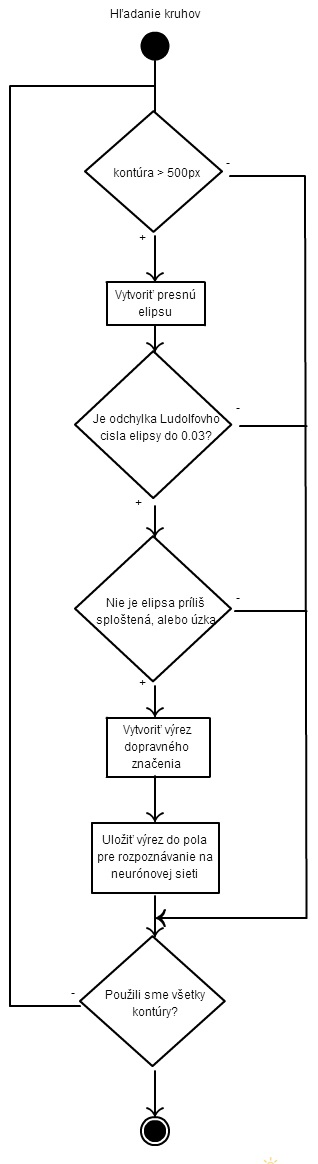
\includegraphics[width=0.4\textwidth,natwidth=318,natheight=1164]{hladanie_kruhov.jpg}
%%	\end{center}
%%	\vspace{-20pt}
%%  	\caption{Algoritmus vyhľadávania kruhov}
%%  	\vspace{-10pt}
%%  	\label{hladanie_kruhov}
%%\end{wrapfigure}
\begin{figure}[p]
\centering
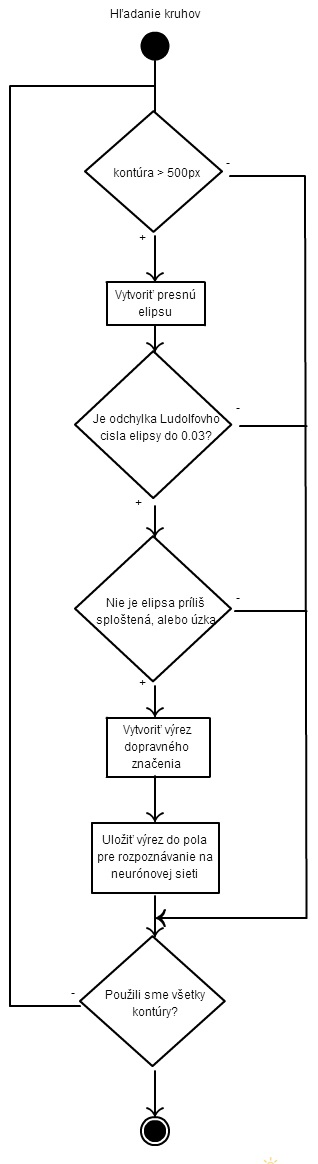
\includegraphics[width=0.4\textwidth,natwidth=318,natheight=1164]{hladanie_kruhov.jpg}
\caption{Algoritmus vyhľadávania kruhov}
\label{hladanie_kruhov}
\end{figure}
- Keďže v predchádzajúcej kapitole sme si navrhli riešenie, ktoré nám vracia len kontúry hľadanej farby, môžeme pokračovať od tohto bodu.
Ako prvé si spravíme cyklus, ktorým budeme prechádzať všetky naše vyhľadané kontúry farieb. Aby sme eliminovali počet prebytočných kontúr, 
je potrené spracovávať čo najrelevantnejšie výsledky. Tento úkon vykoná metóda \emph{contourArea}, vďaka ktorej budeme posielať na ďalšie spracovanie len kontúry väčšie ako 500 pixelov.
\linebreak
\linebreak
- Vzhľadom na to, že výsledky, ktoré dostávame ešte nemôžeme nazvať elipsami, musíme si naše kontúry na elipsy upraviť.
Tento úkon vykonáva metóda \emph{fitEllipse}, ktorá upraví kostrbaté kontúry, ktoré sa aspoň trochu podobajú elipse, na matematicky presnú elipsu.
\linebreak
\linebreak
- Keď už máme detekované elipsy, nastáva posledný krok, a tým krokom je, určiť si toleranciu elipsy dopravného značenia, ktorú vyhľadávam.
Táto tolerancia, je vlastne tolerancia nepresnosti, pri výpočte Ludolfovho čísla. 
Ďalším krokom je tak výpočet už spomínaného ludolfovho čísla a následné overenie jeho nepresnosti. 
Pokiaľ je výsledná hodnota vyhovujúca, nájdený objekt vyrežeme, a zasielame na rozpoznanie neurónovej sieti, ktorá zistí o akú značku sa presne jedná.
\linebreak
\linebreak
Výpočet Ludolfovho čísla:
\begin{align*}
          \pi = \frac{o}{d} \\
\end{align*}
Úprava výpočtu Ludolfovho čísla pre elipsu:
\begin{align*}
          p = \frac{o}{d} = \frac{o}{(\frac{1}{2} y) * ( \frac{1}{2} x)} \\
\end{align*}
Získanie tolerancie:
\begin{align*}
          \pi - p < 0.03 \\
\end{align*}
%%vzorec
%%citacie z knih matematiky
- Pre určovanie tolerancie elipsy, je možné použiť ešte jednu metódu, a tou je overovanie podľa osí. 
Pokiaľ je x-ová os dvoj-násobne väčšia ako y-ová, ide už o elipsu, ktorú by sme ďalej len ťažko identifikovali. 
Takýto nežiaduci stav môže nastať, pokiaľ sa na značku pozeráme na dopravné značenie z príliž veľkého uhlu.
\linebreak
\linebreak
Dva nežiaduce stavy tvaru dopravného značenia:
\begin{align*}
		  \text{ 1.) }
          \frac{\frac{1}{2} x}{\frac{1}{2} y} > 2  \\
          \text{ 2.) }
          \frac{\frac{1}{2} y}{\frac{1}{2} x} > 2  \\
\end{align*}
\subsubsection{Návrh algoritmu pre detekciu trojuholnikov}
\subsubsection{Návrh algoritmu pre detekciu štvorcov}
\subsection{Návrh objektov - UML}
\subsection{Návrh užívteľského prostredia}

\section{Implementácia}
\subsection{Inštalácia Opencv pre Android}
\subsection{Android aplikácia a GUI}
\subsection{Objekty}
\subsubsection{Trieda 1}
\subsubsection{Trieda 2}
\subsubsection{Trieda 3}

\section{Výsledky aplikácie}
\subsection{Detekcia kruhových značiek}
\subsubsection{Značky modrej farby}
\subsubsection{Značky červenej farby}

\section{Záver}

\bibliography{bach}
\bibliographystyle{plain}

\end{document}
